%FRACTIONS AS PARTS OF A WHOLE - WORKSHEET 3
\documentclass[12pt, letterpaper, fleqn]{article}

% ----------------------------------------------------------
% PACKAGES
% ----------------------------------------------------------
\usepackage{graphicx}
\usepackage{xcolor}
\usepackage[most]{tcolorbox}
\usepackage{amsmath, amssymb}
\usepackage{fancyhdr}
\usepackage[utf8]{inputenc}
\usepackage[T1]{fontenc}
\usepackage{enumitem}
\usepackage{geometry}
\usepackage{tikz}
\usepackage{needspace}
\usepackage{multicol}

\usetikzlibrary{arrows.meta, calc, shapes.geometric}

% ----------------------------------------------------------
% PAGE SETUP
% ----------------------------------------------------------
\usepackage{times}
\geometry{letterpaper, top=1.25in, bottom=1.25in, marginpar=0.5in}

% ----------------------------------------------------------
% HEADER / FOOTER
% ----------------------------------------------------------
\newcommand{\logowidth}{3cm}
\setlength{\headheight}{20pt}
\setlength{\footskip}{40pt}

\pagestyle{fancy}
\fancyhf{}
\fancyhead[C]{\small\bfseries Fractions as Parts of a Whole}
\fancyfoot[L]{\raisebox{2pt}{
\includegraphics[width=\logowidth]{../kss.png}}}
\fancyfoot[C]{\thepage}
\fancyfoot[R]{3.14.3}

\renewcommand{\footrulewidth}{0.2pt}

% ----------------------------------------------------------
% THEME COLOR
% ----------------------------------------------------------
\definecolor{customteal}{HTML}{2fbdb9}

% ----------------------------------------------------------
% HELPER MACROS
% ----------------------------------------------------------
\newcommand{\blank}{\underline{\hspace{2.2cm}}}
\newcommand{\blanklong}{\underline{\hspace{6.5cm}}}
\newcommand{\blankshorter}{\underline{\hspace{1.5cm}}}

% ----------------------------------------------------------
% DOCUMENT
% ----------------------------------------------------------
\begin{document}

\textbf{Name:} \underline{\hspace{5cm}}
\hfill
\textbf{Date:} \underline{\hspace{3cm}}\\

\begin{tcolorbox}[colback=customteal!20]
    \large\textcolor{black}{\textbf{Quiz: Fraction Models}}
\end{tcolorbox}

\vspace{5mm}
\begin{enumerate}[itemsep=3cm, leftmargin=0.6cm]
\item Shade the shapes to match the given fraction:
  \begin{itemize}[itemsep=1.5cm]
    \item Shade $\dfrac{3}{4}$: \\
      \begin{tikzpicture}[scale=0.8]
      \draw[thick] (0,0) rectangle (4,1);
      \foreach \x in {1,2,3} { \draw[thick] (\x,0) -- (\x,1); }
      \end{tikzpicture}
    \item Shade $\dfrac{1}{3}$: \\
      \begin{tikzpicture}[scale=0.8]
      \draw[thick] (0,0) circle(1);
      \foreach \a in {90,210,330} { \draw[thick] (0,0) -- (\a:1); }
      \end{tikzpicture}
  \end{itemize}

\item What is the denominator of the fraction $\dfrac{5}{8}$? \blank
\end{enumerate}

\end{document}
